\section{Ejercicio 2}

\subsection{Introducción}
Este ejercicio consiste en entrenar una red neuronal que aprenda a predecir los valores de calor y refrigeracion para un edificio, dado un set de datos
con caracteristicas de cada edificio. A diferencia del Ejercicio 1, se deberá entrenar un modelo de regresión ya que la red tiene que devolver valores
numericos y no clases.

\subsection{Experimentación}
Para los siguientes experimentos se utilizo una arquitectura de red con la siguiente topologia: 8 entradas, 1 capa oculta de 16 unidades y 2 unidades de salida,
tal como se muestra en la figura a continuación.

\begin{figure}[H]
  \includegraphics[width=12cm, height=5cm]{../plot/10-18-2.pdf}
  \centering
  \caption{Red (9-17-2)}
\end{figure}

Cabe destacar que todos los experimentos se corrieron con parametros $\eta$ = 0.02, 500 epocas y un modo de entrenamiento estocastico.
\subsubsection{Experimento 1}
Para este experimento se decidió evaluar el efecto de preprocesar tanto los valores de entrada como de salida de la red propuesta a fin de observar su
comportamiento. Se utilizaron funciones de activacion sigmoidea para la primer capa y lineal para la salida (debido a que la salida debe estar entre 0 y 50 aproximandamente,
 sin normalizar la salida). El preprocesado consistió en restarle a cada muestra la media y luego dividirlo por la varianza, es decir que por cada valor de la entrada
como de salida se lo reemplazo por la siguiente formula:
\begin{equation}
  \dot{x_{i}} = (x_{i} - \mu_{input}) / \sigma_{input}
\end{equation}

\begin{equation}
  \dot{y_{i}} = (y_{i} - \mu_{output}) / \sigma_{output}
\end{equation}

Los resultados obtenidos se presentan a continuacion:

\begin{figure}[H]
  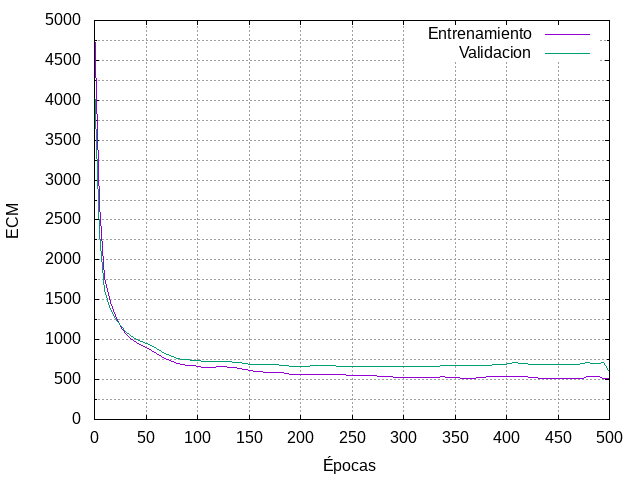
\includegraphics[width=125mm]{imagenes/ej2/ex_1-1_red-9-17-2_errors.png}
  \caption{Con preprocesamiento de entrada}
\end{figure}

\begin{figure}[H]
  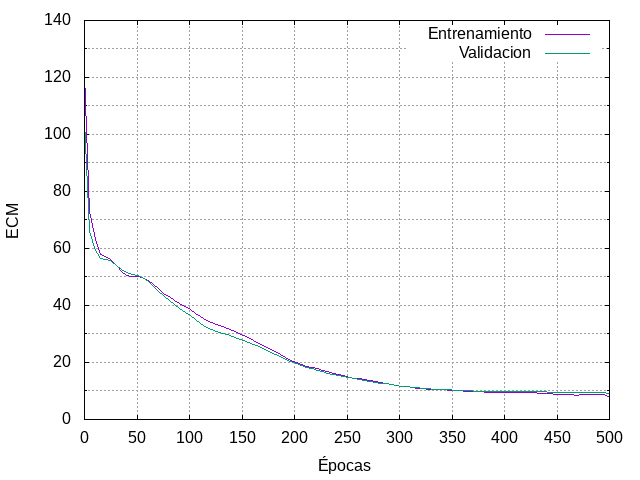
\includegraphics[width=125mm]{imagenes/ej2/ex_1-2_red-9-17-2_errors.png}
  \caption{Con preprocesamiento de entrada y de salida}
\end{figure}

Se observó una amplia diferencia entre ambos entrenamientos ya que el ECM es mucho menor en el caso en que se preprocesa la salida, llegando
a minimos muy diferentes. Con este experimento se evidencia la importancia del preprocesamiento de los datos de entrenamiento.

Debido al peso de estos resultados se decidió seguir entrenando sobre la misma red y preprocesando la salida.

\subsubsection{Experimento 2}
Este experimento consistió en variar las funciones de activacion de la capa oculta. Se decidieron utilizar funciones de tipo \textit{Tangente hiperbolica} y \textit{ReLu}
para analizar comportamientos y performance de la red. Los resultados que se obtuvieron fueron los siguientes:

\begin{figure}[H]
  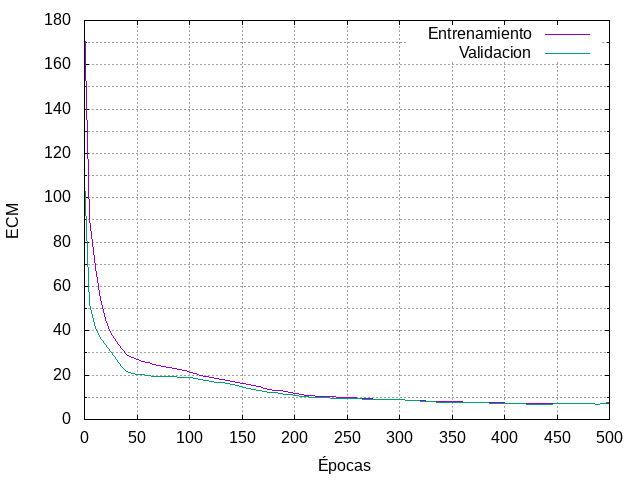
\includegraphics[width=125mm]{imagenes/ej2/ex_2-1_red-9-17-2_errors.png}
  \caption{Funcion de activacion Tangente Hiperbolica}
\end{figure}

\begin{figure}[H]
  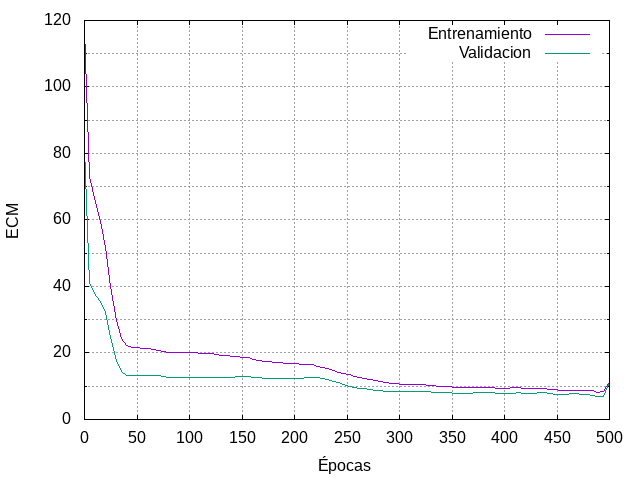
\includegraphics[width=125mm]{imagenes/ej2/ex_2-2_red-9-17-2_errors.png}
  \caption{Funcion de activacion ReLu}
\end{figure}

Se observó que los resultados son bastantes similares, dado que ambas funciones de activación se compartan parecido. Sin embargo, la Tangente hiperbolica tiene un poco menos
de ECM que la ReLu, es por esto que se decidió continuar utilizando la función de activacion de Tangente hiperbolica para la experimentación restante.

\subsubsection{Experimento 3}
Para este experimento se decidió variar la funcion aleatoria de generacion de pesos de la red. Se utilizó una distribución uniforme en el rango (-D, D), donde:
\begin{equation}
  D = \frac{1}{\sqrt{i + o}} \mbox{con i= cantidad de entradas de la capa y o = cantidad de salidas de la capa}
\end{equation}

\begin{figure}[H]
  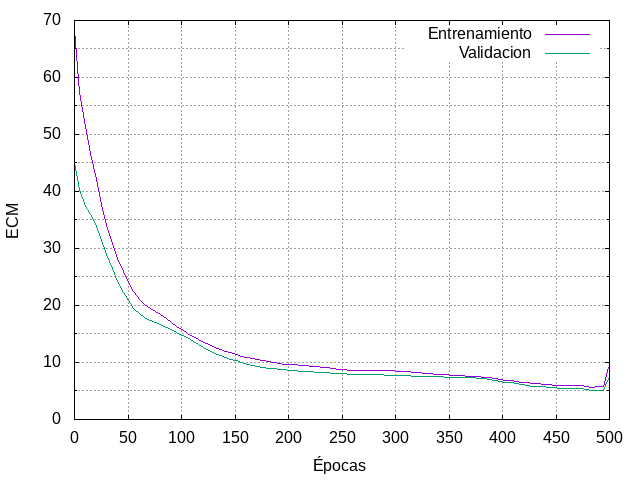
\includegraphics[width=125mm]{imagenes/ej2/ex_3-1_red-9-17-2_errors.png}
  \caption{Con preprocesamiento de entrada}
\end{figure}

\begin{figure}[H]
  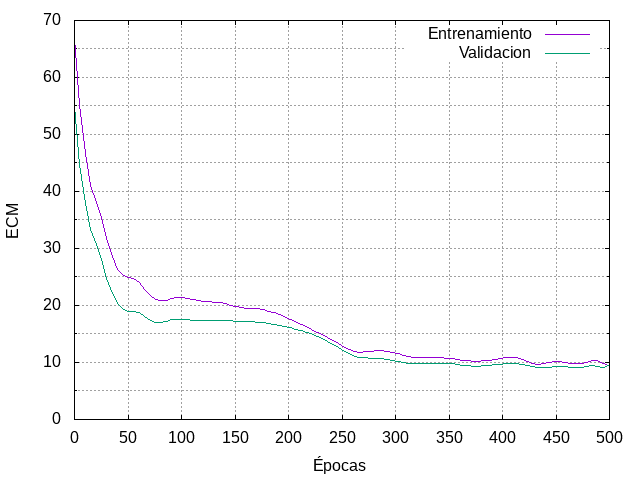
\includegraphics[width=125mm]{imagenes/ej2/ex_3-2_red-9-17-2_errors.png}
  \caption{Con preprocesamiento de entrada y de salida}
\end{figure}
\subsection{Conclusión}

\newpage
